% Indicate the main file. Must go at the beginning of the file.
% !TEX root = ../main.tex

%----------------------------------------------------------------------------------------
% CHAPTER TEMPLATE
%----------------------------------------------------------------------------------------

\chapter{Results and discussion} % Main chapter title
\label{Chapter4}
The approach used in this work of modelling spectra and training a neural network model on the structure-label relation is an inherently biased approach, as we add the prior assumption of the model to create accurate spectra. Although this is clearly not the preferred baseline, scarce availability of labelled data often forces one to accept trade-offs. Nevertheless, this does not immediately imply failure at our tasks, but more importantly strongly depends on the prior assumption of spectra modelling. The following structure resembles our tasks formulated in the \nameref{Chapter1}. For each task, a table with the respective models, datasets and accuracies is shown.

%----------------------------------------------------------------------------------------
% SECTION 1
%----------------------------------------------------------------------------------------
\section{Qualitative elemental identification of bilayer systems}
\subsection{Elemental identification}
% model performance
The model performance for the qualitative elemental identification is shown in Table \ref{tab:acc_qual}. The categorical accuracies were computed for the individual clean and the mixcont dataset. Because experimental data can contain contamination, we generally expect the mixcont dataset to make our model more robust in that respect.
During the model development, it was obvious that we are prone to overfitting the simulated data resulting in poor performance on test data. Especially, because we do not represent the experimental spectra with enough accuracy, we must make sure to focus on the robustness of the model. Thus, the obvious approach was to choose the most simple model which was able to train effectively without overfitting and before aiming at the highest accuracy rates. The models remained unchanged for the qualitative identification for all datasets. Thus, a total of 8 models were developed for task 1 - one of each model type for each layer and the models were trained on the three datasets. For each best performing model for each layer and dataset, the confusion matrices are shown.

\begin{table}[H]
    \centering
    \centerline{
    \begin{tabular}{c|c|c|c|c|c|c}
        Dataset & Layer & Model   & No. Parameters & Training set acc. & Validation set acc. & Test set acc.*    \\
        \hline 
        mixcont & top   & CNN     &  82.1 M        &    91.34      &    86.58       & 24.65          \\
        (n=272k)&       & CNN-DCT &  85.5 M        &    97.25      &    86.42       & 38.5           \\
                &       & CBAM    &  20.1 M        &   92.80       &    82.80       & 28.64          \\
                &       & ViT     &  25.8 K        &    79.92     &    82.69       &  52.56  \\
        \hdashline
                & bot   & CNN     &   82.1 M       &    89.05       &      79.64    &     45.12      \\
                &       & CNN-DCT &                &               &                &                 \\
                &       & CBAM    &                &               &                &                \\
                &       & ViT     &                &               &                &               \\
        \hline                                   
        clean   & top   & CNN     &                &               &                &            \\
        (n=65k)&       & CNN-DCT &                &               &                &            \\
                &       & CBAM    &                &               &                &            \\
                &       & ViT     &                &               &                &            \\
        \hdashline
                & bot   & CNN     &                &               &                &             \\
                &       & CNN-DCT &                &               &                &             \\
                &       & CBAM    &                &               &                &            \\
                &       & ViT     &                &               &                &            \\
    \end{tabular}}
    \caption{Categorical accuracies, and number of parameters of the models in respect to dataset and sample layer
    *Test Dataset n=\nelementalspectra}
    \label{tab:acc_qual}
\end{table}



\subsubsection{Top layer prediction}
The best model to predict the top layer element was the Vision Transformer-Model, with an accuracy on the test dataset of 52.56 \%. Figure \ref{fig:top_best_loss} shows the categorical crossentropy loss and categorical accuracy for the training (blue) and the validation (orange) datasets respectively. In the confusion matrix, we can see that in the test dataset, Iron (Fe) has been wrongly predicted as Lithium (Li) a total of 4 times, which are the most failures of any wrongly predicted elements. An approach would be to plot the attention of the model on Lithium and Iron spectrum data to investigate the reason behind. However, as shown in Figures \ref{att:Fe} and \ref{att:Li}, they are not similar at all, which suggests that the model lacks complexity as both cases overlap in the feature space. As the model only has 25.8k trainable parameters, this is very much possible. 

\begin{figure}[H]
    \centering
    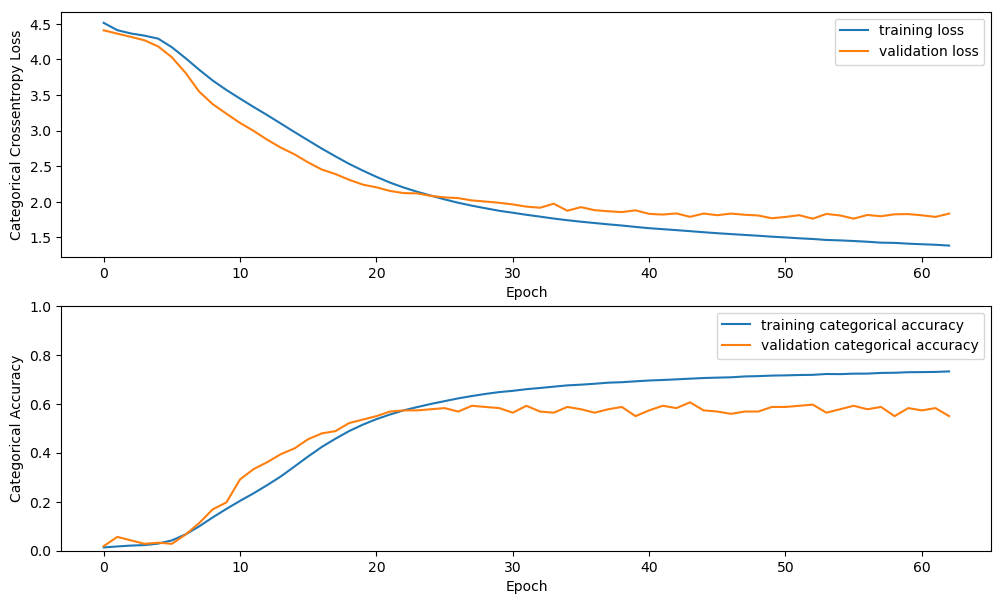
\includegraphics[width=\textwidth]{Figures/top_best_loss_acc_vit_4_32_3_4_64.png}
    \caption{Categorical crossentropy loss and crossentropy accuracy for the ViT model training on top-layer training data-labels}
    \label{fig:top_best_loss}
\end{figure}

\begin{figure}[H]
    \centering
    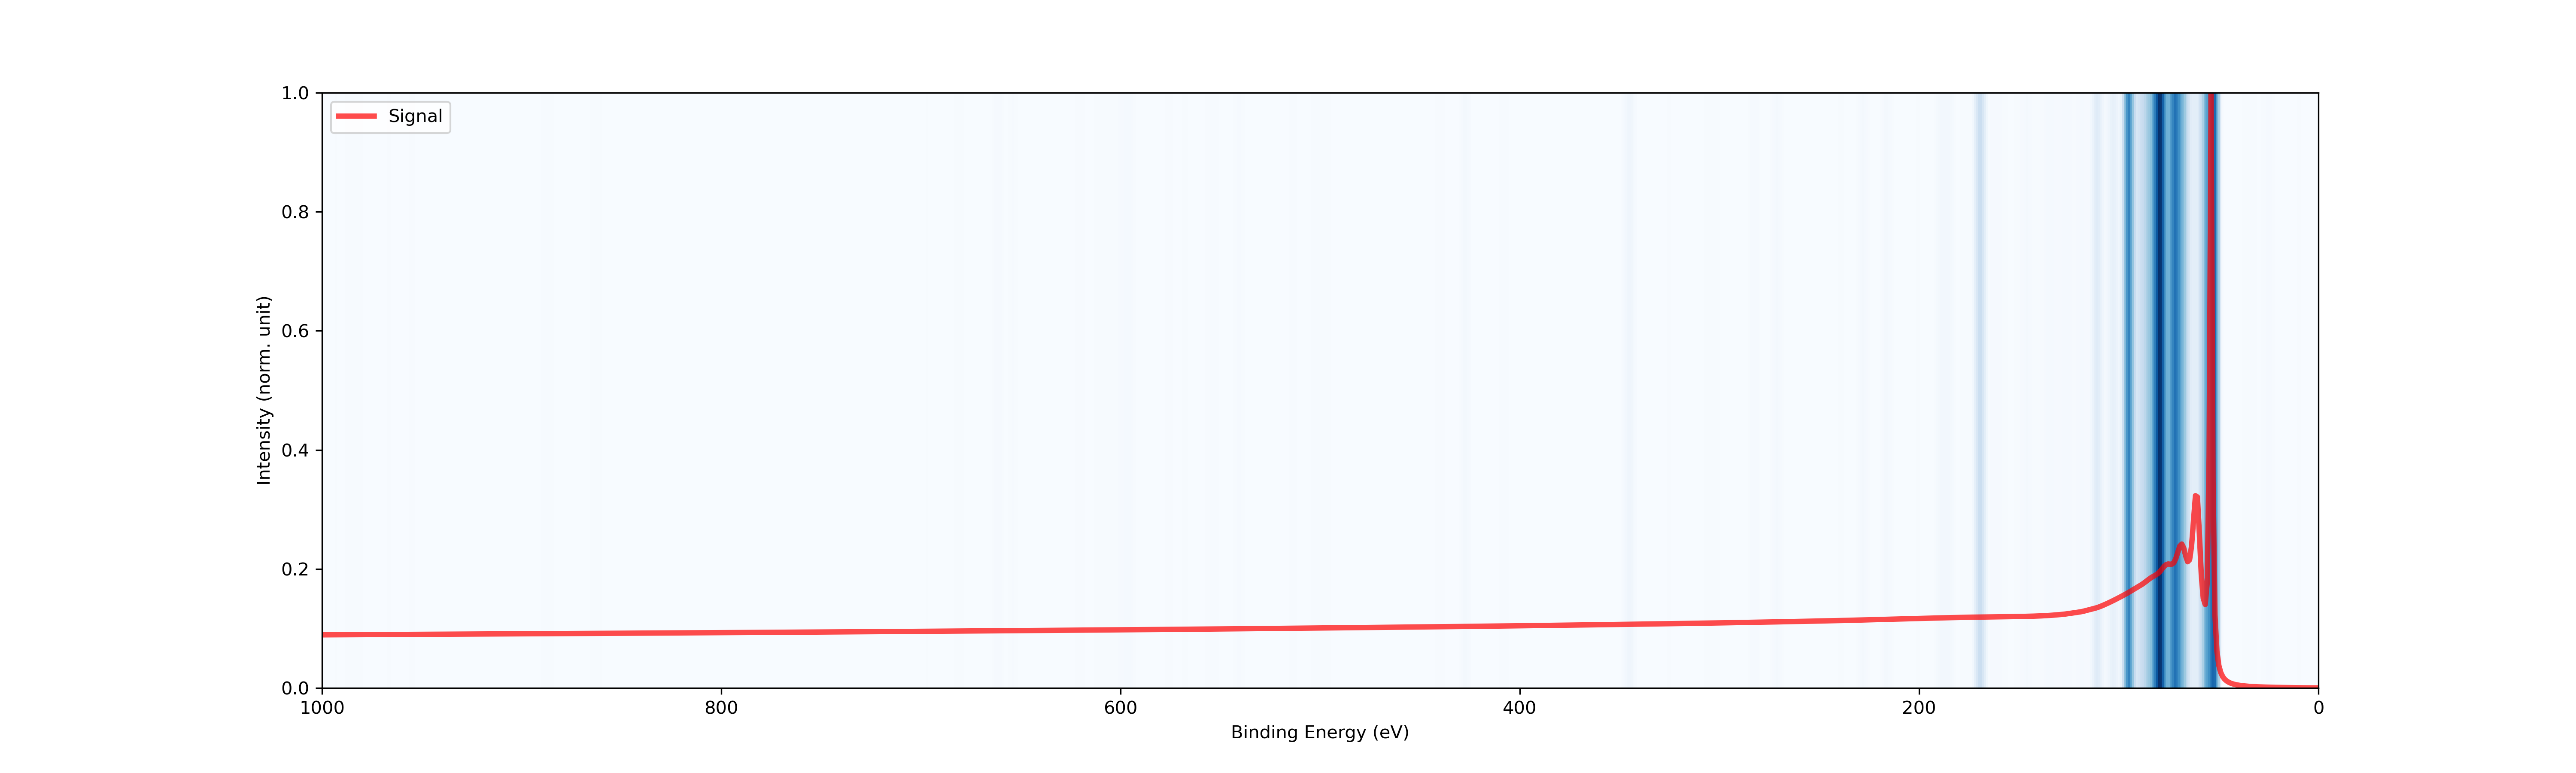
\includegraphics[width=\textwidth]{Figures/attention_map_Li.png}
    \caption{Attention map (blue) for the Lithium spectrum (red) prediction}
    \label{att:dy}
\end{figure}
\begin{figure}[H]
    \centering
    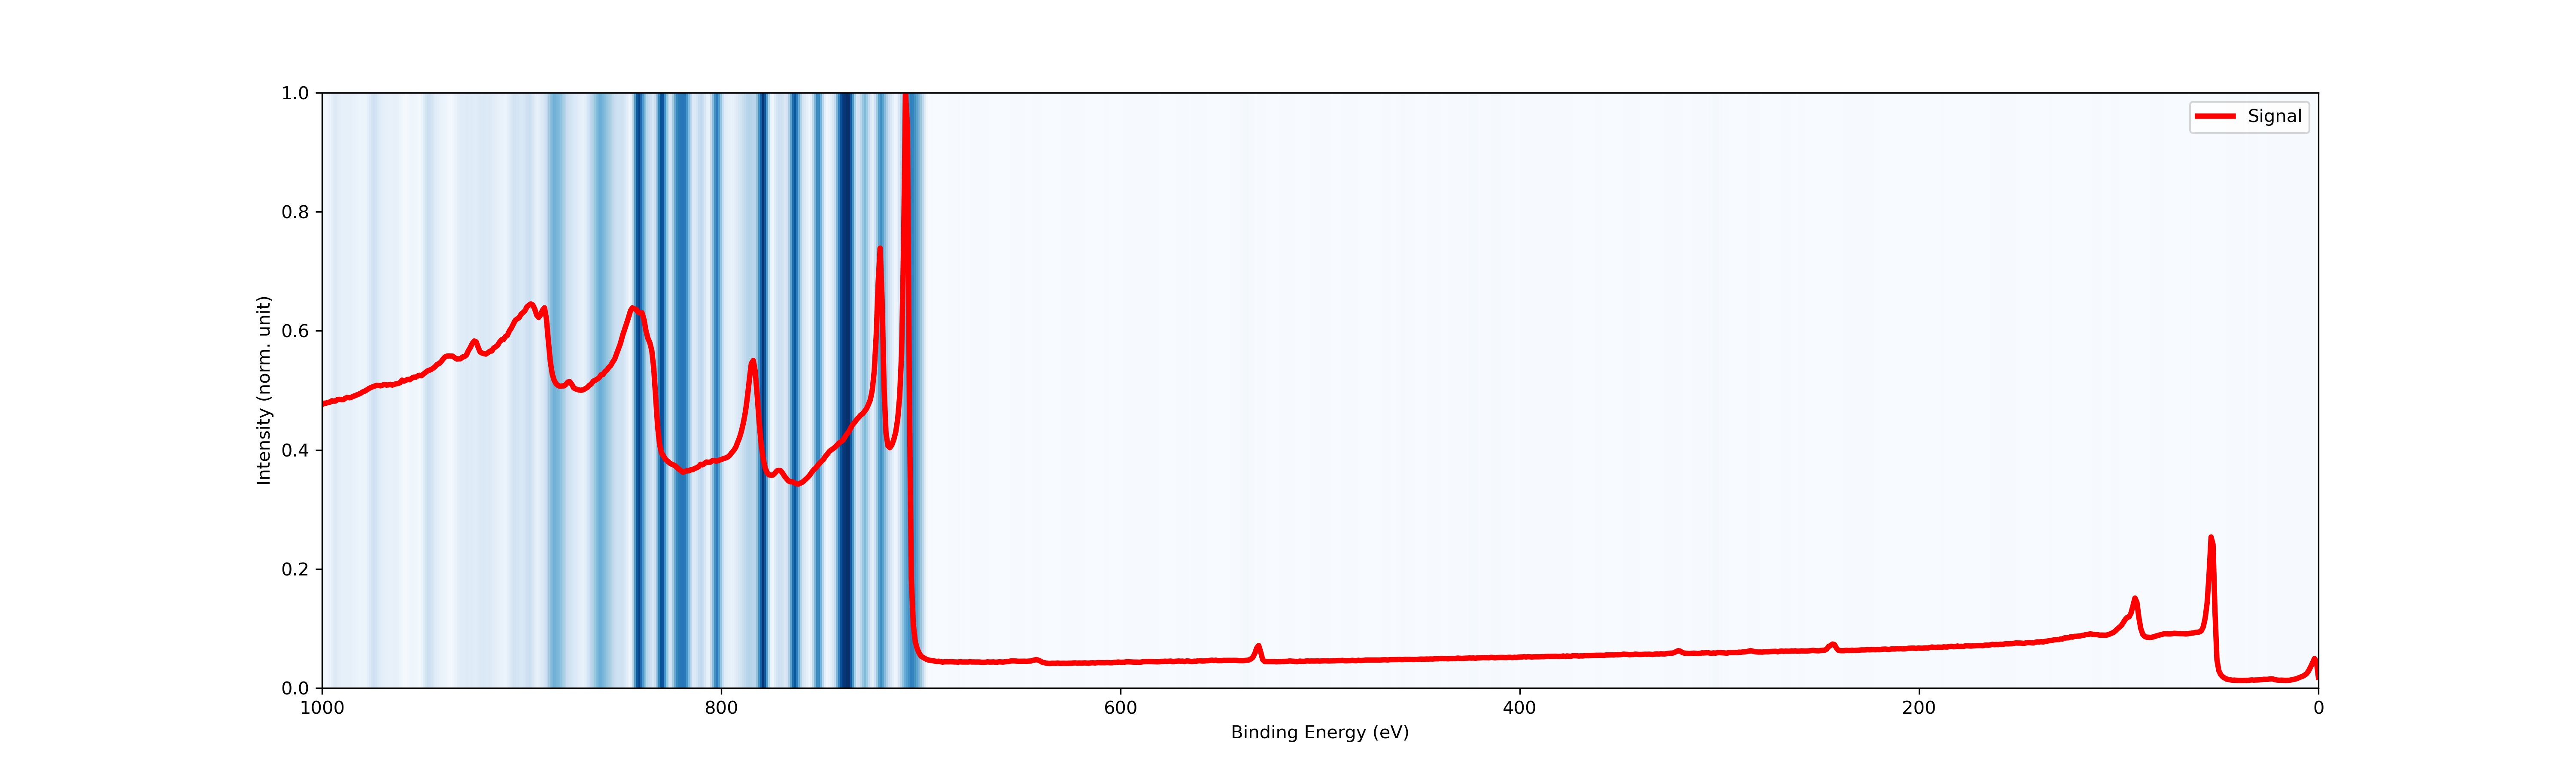
\includegraphics[width=\textwidth]{Figures/attention_map_Fe.png}
    \caption{Attention map (blue) for the Iron spectrum (red) prediction}
    \label{att:c}
\end{figure}




\begin{center}
\begin{figure}[H]
        \centerline{\includegraphics[width=1.4\textwidth]{Figures/best_task_1_model_CM.png}}
    \centering
    \caption{Confusion Matrix of Test-Data for best Top-Layer prediction}
    \label{cm_cnn_1l}
\end{figure}
\end{center}



\subsubsection{Bot layer prediction}


From the experimental data, the same test dataset was used as for the top-layer prediction. Because survey scans of buried layers are rare, we considered pure elemental spectra to be composed of a buried layer of the pure element respectively.
From Table \ref{tab:acc_qual}, we can see that the performance of the bottom layer prediction is not always lower than the top layer prediction. However, we would expect a lower accuracy for the bottom layer, due to the principle of XPS measurement, as electrons from the deeper layer must travel through the top layer and thus will be less intense and more influenced by scattering from interactions. Anyway, as we consider experimental data from pure elements as a two-layer system in our test-set, it could also be that the simulated spectra from buried pure elements actually resembles ground truth more accurately.




\subsection{Depth profile determination of native oxides and elements}

% As there's almost no test data this is experimental
Depth profiling or determination of overlayer thickness is often conducted in scientific experiments. However, data is usually not publicly available - and if - it does often not include survey spectra. This is because these measures are usually done with ion-sputtering profiling or angle-resolved measurements and as these experiments are time-consuming, only the regions of interests (where the peaks are expected depending on the sample) are scanned.
As depth profiling data is not readily available from public databases, the datasets obtained internally as explained in chapter \ref{exp_depth}, were used to evaluate the model on experimental data.
% model performance

\begin{table}[H]
    \centering
    \begin{tabular}{c|c|c|c|c}
        Dataset & Model   & No. Parameters & Training Dataset    & Validation Dataset    \\
        \hline
 mixcont+oxides& CNN     &                &                       &                         \\
               & CNN-DCT &                &                       &                         \\
               & CBAM    &                &                       &                         \\
               & ViT     &                &                       &                         \\

    \end{tabular}
    \caption{ and number of Parameters of the models in respect to dataset and layer}
    \label{tab:acc_depth}
\end{table}

% experimental data (AG_AG etc.)




%----------------------------------------------------------------------------------------
% SECTION 2
%----------------------------------------------------------------------------------------
\section{Elemental quantification of single layer systems}

% model performance
The model performance for the quantitative assessment of chemical composition is shown in Table \ref{tab:acc_quant}. The mean squared errors were computed for the multi dataset for each model.
% experimental data (AG_AG etc.)
From all experimental data, $\nmultispectra$ elemental spectra were used for the quantitative prediction. 

\begin{table}[H]
    \centering
    \begin{tabular}{c|c|c|c|c|c}
       Dataset & Model   & No. Parameters & Training dataset & Validation dataset*  & Test dataset*    \\
        \hline
        multi  & CNN     &   9.1 M        &     35.5       &   25.95                 &  1.92      \\
               & CNN-DCT &  35.3 M        &    13.61          &    14.16            &    3.83   \\
               & CBAM    & 28.2 M         &    23.32         &    14.94             &  2.68   \\ % CBAM_512_3_ES_MAE_4
               & ViT     &   35.3 M     &    33.81       &      34.86    &   2.68        \\
    \end{tabular}
    \caption{Number of parameters and threshold accuracy of the models}
    \label{tab:acc_quant}
\end{table}

As the threshold accuracy represents the percentage of elements with >10\% proportional content correctly quantified within a $\pm$10\% relative margin, it can be well compared to an experienced researchers result. With a maximum threshold accuracy of 3.83\% however, we are far off a good result for our best model. The full prediction mapped as heatmap is shown in Figure \ref{fig:multi_best_model}

\begin{figure}
    \centering
    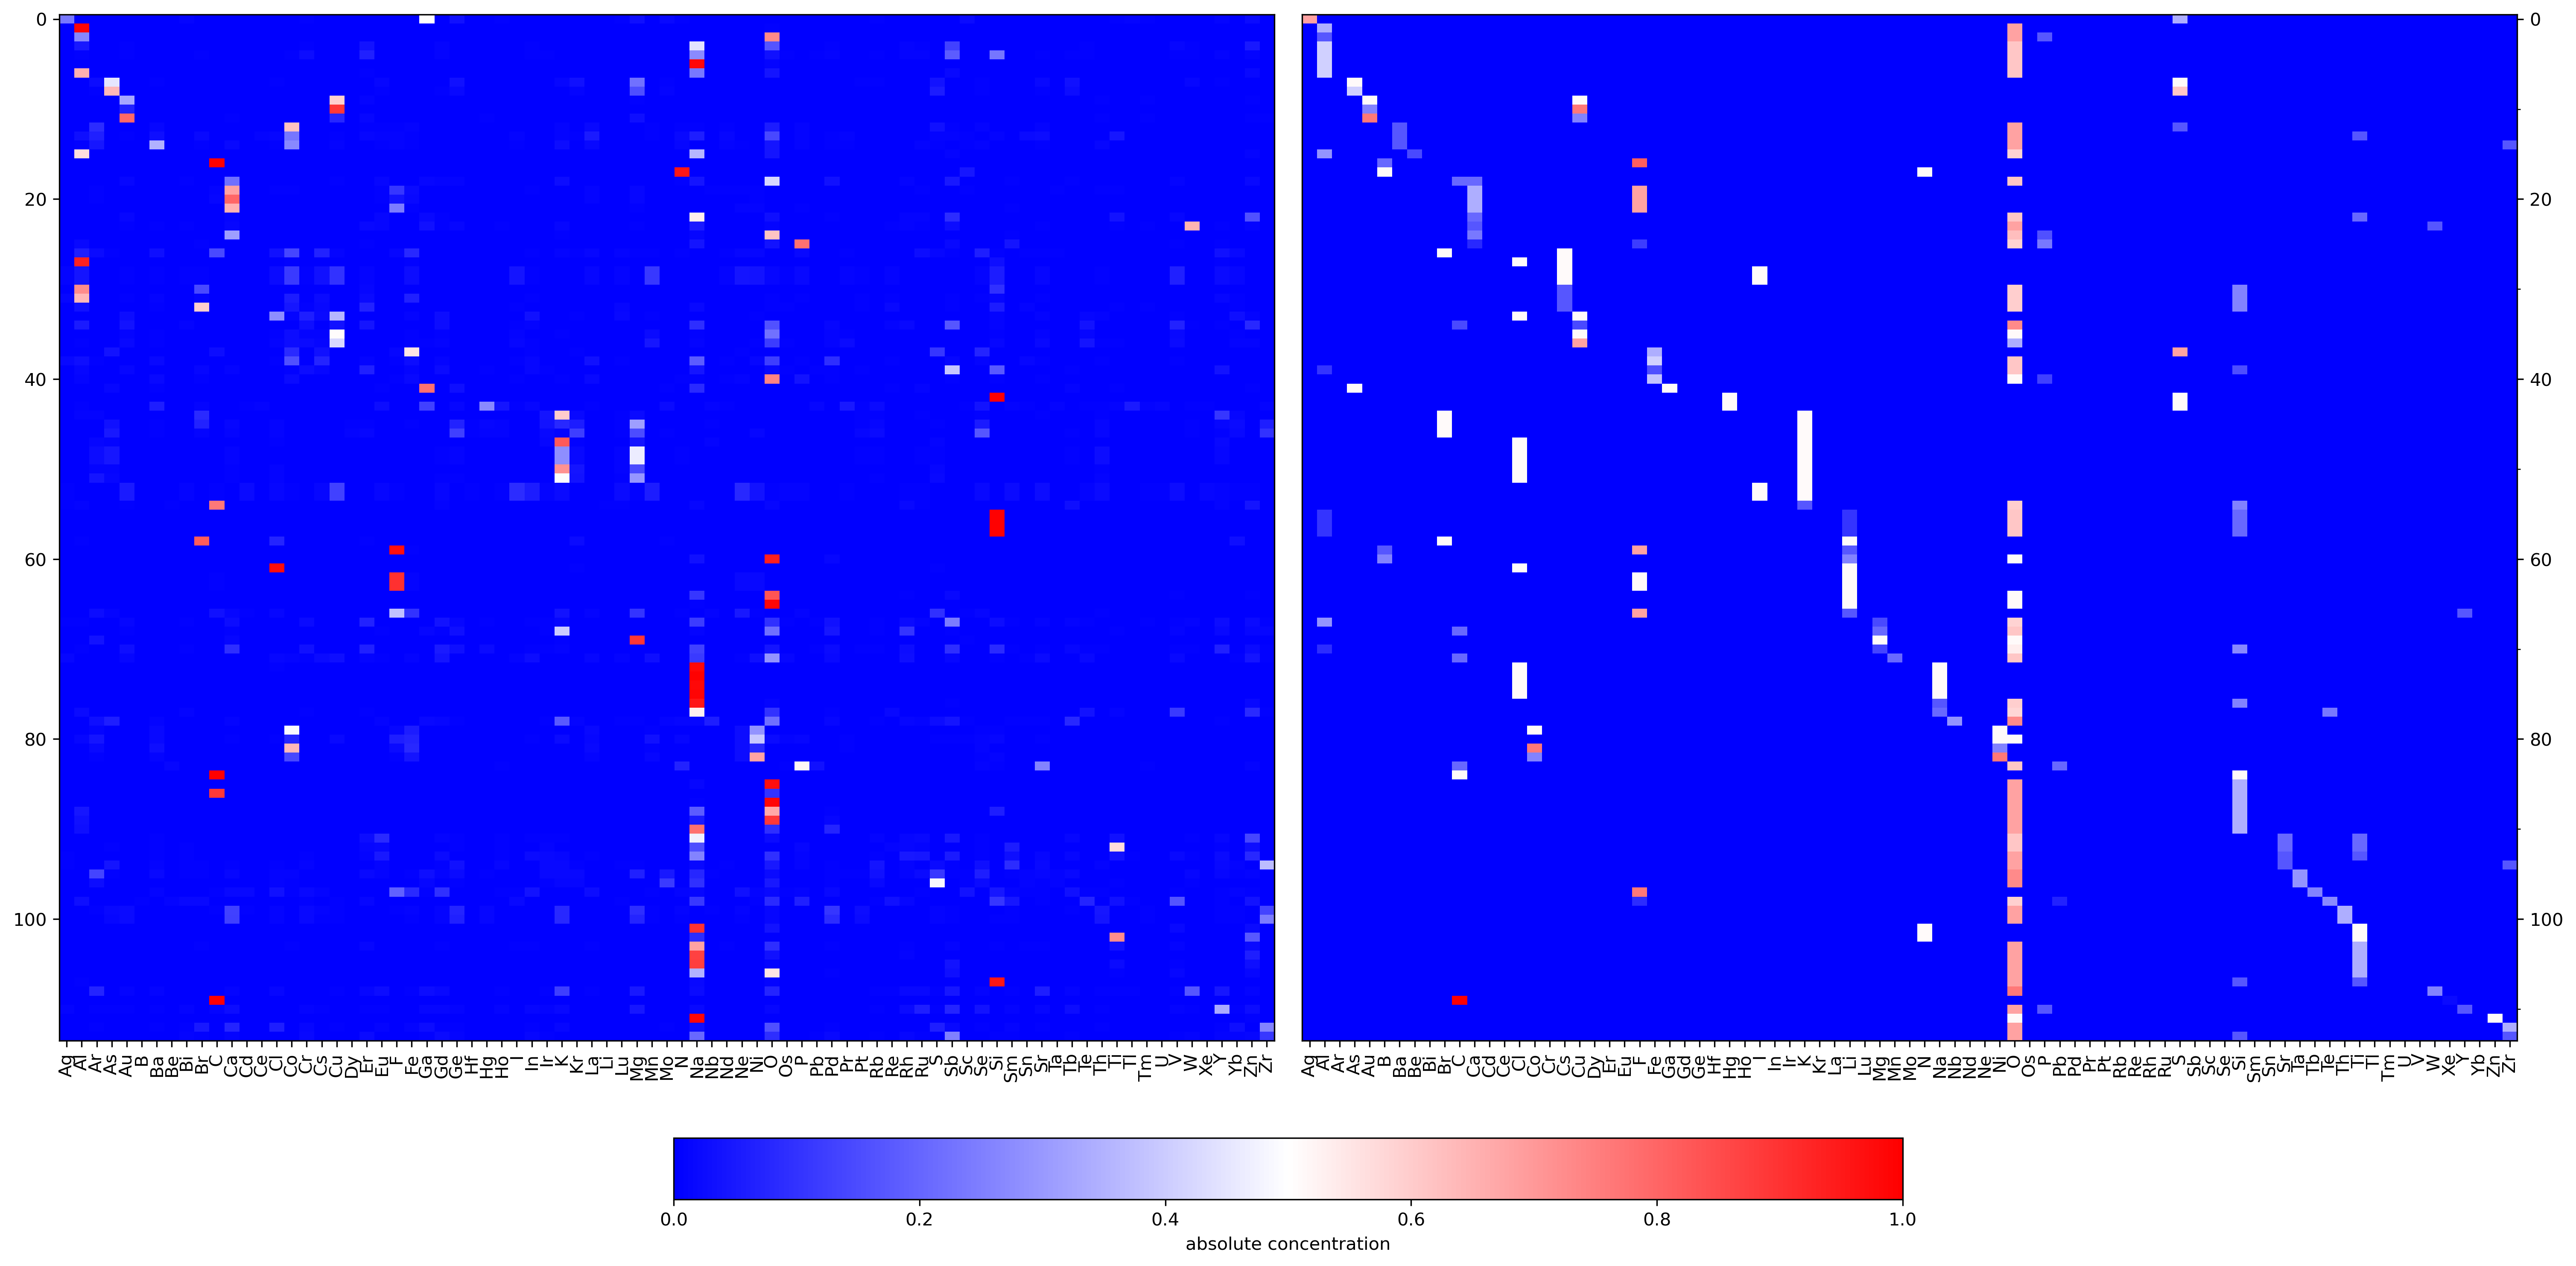
\includegraphics[width=\textwidth]{Figures/cnn_dct_mae_32F_multi_best_model_pred.png}
    \caption{The predictions of the best performing model on experimental multi-component data}
    \label{fig:multi_best_model}
\end{figure}

In contrast to previous studies on deep-learning assisted quantitative XPS analysis \cite{drera_deep_2019}, no relative sensitivity factors were applied in this approach. Furthermore, a significantly smaller training dataset of 30k versus the 100k which were used in their work. Lastly, the test data spectra they used were collected in experimental conditions and the training dataset was simulated according to the known conditions.

% plot visual attention feature

